%This is the Preface
%%=========================================
\addcontentsline{toc}{section}{Preface}
\section*{Preface}

Internet of Things (IoT) applications very often involve use of sensors. Motion sensing can be used in a vast amount of applications and are therefore very interesting in high volume IoT products. Replacing a battery in such an application is often undesirable, and may even in some cases be impossible. It is therefore essential for such applications to have sensors that consumes as little power as possible. This project thesis elaborates on different techniques to acquire data from an accelerometer at the lowest possible power consumption. 

The project is carried out for a Norwegian company called Disruptive Technologies in conjunction with the Norwegian University of Science and Technology.

%Here, you give a brief introduction to your work. What it is (e.g., a Master's thesis in RAMS at NTNU as part of the study program xxx and\ldots), when it was carried out (e.g., during the autumn semester of 2021). If the project has been carried out for a company, you should mention this and also describe the cooperation with the company. You may also describe how the idea to the project was brought up.\\[2cm]

\begin{center}
Trondheim, 2015-12-16\\[1pc]
\begin{figure}[h]
\centering
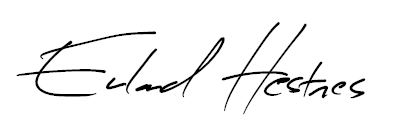
\includegraphics[scale=0.5]{fig/underskrift.png}
\label{fig:underskrift}
\end{figure}
Erlend Hestnes
\end{center}